\section{Svolgimento}
\subsection{Analisi del problema}
Abbiamo iniziato analizzando le richieste del problema da un punto di vista matematico. Per risolverle, bisogna essere in grado di trovare i documenti che contribuiscono all'incremento del fatturato e discriminare gli altri. In un secondo momento, è necessario calcolare la media (Eq.\ref{eq:media}) e la varianza (Eq.\ref{eq:varianza}) utilizzando le formule sottostanti.
\begin{equation}
    \bar{x} = \frac{1}{n} \sum_{i=1}^{n} x_i
    \label{eq:media}
    \end{equation}
    
    \begin{equation}
    \sigma^2 = \frac{1}{n} \sum_{i=1}^{n} (x_i - \bar{x})^2
    \label{eq:varianza}
    \end{equation}
    
Successivamente, sarà necessario calcolare l'ammontare del fatturato diviso per ogni mese di ogni anno. Una volta elaborate queste informazioni, si può procedere ad identificare il mese di ogni anno che ha il valore più alto e più basso, analizzandoli tramite le funzioni di minimo e massimo e raggruppando per anno.
\subsection{Analisi del Dataset}
Procediamo con l'analisi del dataset con i comandi
\begin{lstlisting}[language=R]
    summary(df)
    table(df$tipo)
\end{lstlisting}
che vengono utilizzati per valutare la tipologia dei dati e per estrarre i valori della prima colonna riferiti al tipo di documento.
\begin{table}[ht]
\centering
\begin{tabular}{|l|c|}
\hline
Tipo di documento & Quantità \\
\hline
BUONO.PRELIEVO & 2146 \\
DDT & 15 \\
FATTURA & 556 \\
INVENTARIO & 1 \\
NOTA.DI.CREDITO & 9 \\
OFFERTA & 622 \\
PREVENTIVO & 240 \\
RICEVUTA & 11 \\
\hline
\end{tabular}
\caption{Analisi delle tipologie di documento}
\label{tab:esempio}
\end{table}
In prima analisi, ci rendiamo conto che i documenti che apportano incremento al fatturato sono della tipologia fattura e ricevuta. Andiamo quindi ad impostare un filtro che ci aiuta ad estrarre dal dataset i documenti interessati.
\subsection{Risoluzione tramite codice R}
A questo punto, procediamo con il calcolo della media (Allegato contabilita.r) utilizzando la funzione \codeword{aggregate}, aggregando in base ai mesi di ogni anno e applicando la funzione di calcolo della media (\codeword{FUN = mean}). Vengono fatti in seguito delle trasformazioni per estrarre dalla data le informazioni di anno e mese e renderle più facilmente leggibili. Successivamente, andiamo a calcolare la varianza utilizzando la stessa funzione \codeword{aggregate} e impostando \codeword{FUN = var}.


\begin{figure}[ht]
\centering
\begin{minipage}{.3\textwidth}
    \centering
    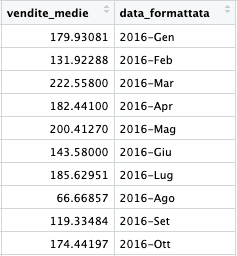
\includegraphics[width=\linewidth]{img/media_r.png}
    \caption{Estratto del dataset con la media}
    \label{fig:immagine1}
\end{minipage}
\begin{minipage}{.3\textwidth}
    \centering
    \end{minipage}
\begin{minipage}{.3\textwidth}
    \centering
    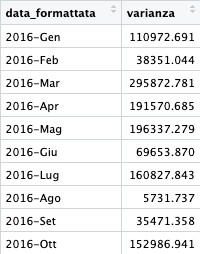
\includegraphics[width=\linewidth]{img/varianza_r.png}
    \caption{Estratto del dataset con la varianza}
    \label{fig:immagine2}
\end{minipage}
\end{figure}
Per la soluzione dei job 3 e 4, si è reso necessario andare a fare un calcolo preliminare, ovvero aggregare le informazioni delle vendite in base al mese e all'anno. Successivamente, si è estratto il valore maggiore (per il job 3) e il valore minore (per il job 4) e visto che si è persa l'informazione specifica del mese, è stato necessario andare a recuperarla facendo un merge con la tabella aggregata precedente e le due tabelle risultanti dall'estrazione dei valori di minimo e massimo.
\begin{lstlisting}[language=R]
    mesi_max = merge(mesi_max_solo_anno, somma_mesi, by="vendite_totali")
\end{lstlisting}
\subsection{MapReduce usando Javascript}
Una volta affrontato il problema con lo scritto in R, andiamo ad analizzare il problema sotto il paradigma di MapReduce. Per una prima analisi, utilizziamo lo strumento del professor Pirrone che permette un rapido approccio a questo modo di scrivere codice. I primi step intrapresi sono andare a dividere il file di input per riga e darlo in pasto allo script di mapping.
La fase di mapping prevede la divisione della linea letta in input e sui tre valori che porta (tipologia ordine, data e costo). Successivamente, andiamo (come fatto in precedenza) a filtrare per la tipologia di ordine fattura e ricevuta: nel caso in cui la tipologia d'ordine appartenga a queste due categorie, viene creata una coppia che ha come chiave la data e come valore l'importo, o costo, del documento.


\begin{lstlisting}[language=Java, caption={Script di mapping}]
    return V_In_Map.map(function(item){
        //scrivo il codice di map
        var tipoOrdine = item.split(",")[0]
        var data = item.split(",")[1]
        var costo = item.split(",")[2]

        var chiave;
        var valore;
        if(tipoOrdine === "FATTURA" ||
        tipoOrdine === "RICEVUTA"){
            chiave = data.slice(0,6);
            valore = costo;
        }
        else
        {
            chiave = "NULL";
            valore = 0;
        }
        return keyVal(chiave, valore);
    });

\end{lstlisting}
Serve fare una precisazione: in un paradigma di MapReduce normale, è possibile scartare dei dati in input. In questo tool, è sempre necessario fornire un output di mapping. Di conseguenza, invece di scartare i documenti che non sono utili al fine del programma, vengono mappati con una chiave "null", che nelle elaborazioni successive non verrà considerata.

Per il primo job (Allegato job1.js) , lo script di reduce andrà a recuperare tutti i valori relativi ad una determinata chiave, ovvero ad una data, e a calcolare la media (andandoli a sommare e successivamente a dividere per il numero di valori associati a quella data).
\begin{figure}[H]
    \centering
    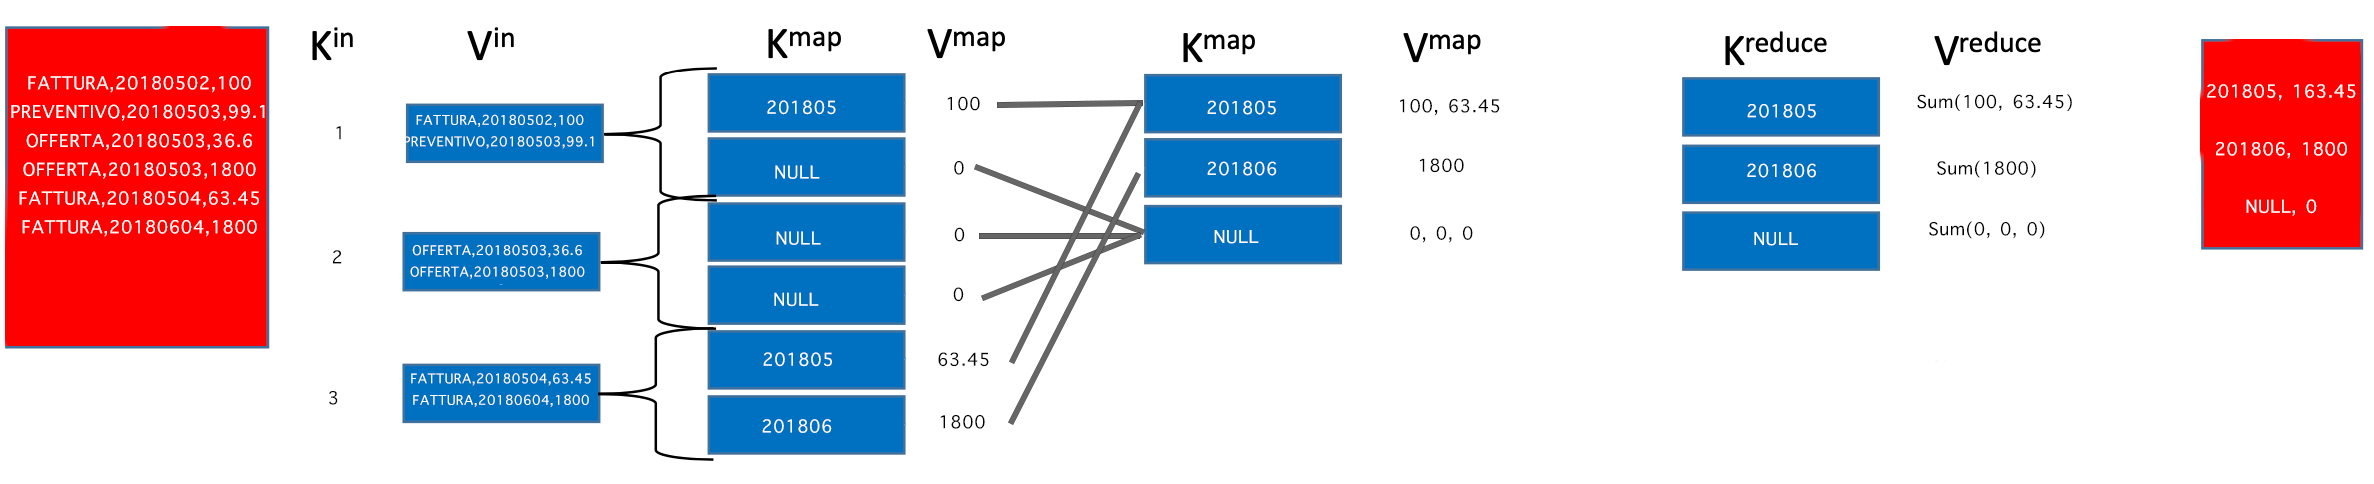
\includegraphics[scale=.15]{img/mapReduceScheme.png}
    \caption{Schema di MapReduce per il primo job}
    \label{figure:mapReduceJob1}
\end{figure}
Nel secondo job (Allegato job2.js), andiamo a riciclare lo stesso script di mapping. Per la fase di reduce, andiamo prima a calcolarci la media di valori associati a quella data (esattamente come il job precedente). Il secondo passaggio è quello di andare a calcolarci per ogni valore lo scarto quadratico rispetto alla media, utilizzando la formula (Eq.\ref{eq:media}, Eq.\ref{eq:varianza}). Come ultimo step, ogni valore di scarto quadratico viene sommato alla media.

Per il job 3 e il job 4, risultano necessari due passaggi del processo di MapReduce:
\begin{itemize}
    \item Il primo passaggio (Allegato prejob34.js) prevede di raccogliere la somma degli importi di ogni mese dell'anno (viene utilizzato parte del codice del primo job senza andare a calcolare la media, ma solo facendo la somma)
    \item Il secondo passaggio prevede un mapping leggermente diverso, dove come chiave viene inserito l'anno e come valore viene inserito sia il mese che la media degli importi. Lo script di reduce andrà a cercare per ogni anno il valore massimo (per il job 3, Allegato job3.js) e il valore minimo (per il job 4, Allegato job4.js) dell'importo in maniera iterativa. Di conseguenza, questo ha permesso di salvare da parte le informazioni relative al mese e di riportarla a fine elaborazione.
\end{itemize}
\subsection{MapReduce usando R e Hadoop}
\subsubsection{Scripting}
Si è quindi passati ad implementare il MapReduce utilizzando script in R sulla piattaforma Hadoop. Per iniziare ad utilizzare la piattaforma, è fondamentale inizializzare le variabili d'ambiente e far partire i servizi per la gestione delle risorse (Yarn) e il file system condiviso (DFS).

Per l'esecuzione del singolo script, vengono fatte altre operazioni preliminari: per ogni script viene prima eliminata e poi ricreata sul file system condiviso la cartella di lavoro (andando così a pulire le tracce delle precedenti elaborazioni). In seguito, viene caricato all'interno del DFS il file che andremo ad utilizzare come input. Finalmente, possiamo andare a lanciare il nostro script utilizzando lo streaming di Hadoop. Come ultimo passaggio, andiamo a visualizzare a schermo l'output prodotto, lo copiamo nell'hard disk locale e lo rinominiamo.

Queste operazioni sono state automatizzate da uno script in Bash (Allegato \texttt{all\_jobs.sh}) e sono state inserite delle chiamate per monitorare le tempistiche e le performance (per salvarle poi in un file).
\subsubsection{Implementazione in R}
Gli script in R prendono spunto da quelli utilizzati prima nel linguaggio Javascript. Lo script di mapping (Allegato mapper.r), come prima, prende il file in input e per ogni riga, estrae il tipo di ordine, la data e il costo, mandando in output solo le tipologie di ordine presenti nel filtro. Come detto già in precedenza, lo script di mapping è univoco per tutti e quattro i job.

Nel primo script di reduce (Allegato \texttt{reducer\_job1.r}), andiamo a sfruttare quelle che sono le peculiarità del paradigma di mappare Douce, andando a creare un nuovo Environment. Successivamente, andiamo a leggere l'output dello script precedente, estrarre per ogni riga la data e l'importo, e controllare se all'interno del nuovo ambiente quella data è già stata inserita:
\begin{itemize}
    \item nel caso il valore della data (mese anno) non fosse presente, viene inserito come importo complessivo l'importo attuale e il conteggio degli elementi viene messo a uno. Il tutto poi viene inserito all'interno dell'ambiente.
    \item Nel caso il valore se è già presente, viene recuperato l'importo complessivo, al quale si somma l'importo attuale, aumentato il conteggio di uno e inserito il tutto nuovamente all'interno dell'ambiente.
\end{itemize}
Una volta ultimato questo processo, si passa ad estrarre dall'Environment tutti i valori inseriti e si procede con un processo di "abbellimento" prima di mandare i dati in output.

Il job 2 (Allegato \texttt{reducer\_job2.r}), nel processo di reduce, ha una peculiarità: oltre ad implementare l'algoritmo per il calcolo della varianza (rispetto a quello di calcolo della media), per recuperare le informazioni relative alle medie, va a leggere all'interno del file system di Hadoop il file di output precedente.

I job 3 e 4 (Allegato \texttt{reducer\_job3.r} e  \texttt{reducer\_job4.r}), invece, nella fase di reduce, salvano all'interno dell'ambiente la somma degli importi raggruppati per data (mese dell'anno). In un secondo momento, queste informazioni vengono recuperate, aggregate per anno ed estratti i valori di massimo e minimo.

In questa fase, ho preferito non dilungarmi nell'analisi dell'algoritmo (visto che gran parte della complessità si è affrontata con i linguaggi precedenti), ma ho preferito dare risalto a quegli aspetti tipici di questo paradigma di programmazione che Hadoop offre.
\subsubsection{MapReduce con Python e Hadoop}
Visto che negli ultimi anni Python si sta affermando come linguaggio di programmazione per la data Science, molti programmi e piattaforme si sono aperti alla compatibilità con esso. Su Hadoop, è infatti possibile sfruttare il paradigma MapReduce facendo scripting, oltre che con R, anche con Java e Python. Ho voluto così tradurre il lavoro fatto fino adesso in R anche in Python (Allegato mapper.py, \texttt{reducer\_job1.py}, \texttt{reducer\_job2.py}, \texttt{reducer\_job3.py}, \texttt{reducer\_job4.py}) e fare una piccola comparazione delle performance di questi due linguaggi. Anche qui, non entro nel merito dell'implementazione, in quanto l'algoritmo è esattamente lo stesso. Cambia solo il linguaggio in cui è scritto.
È stato scritto uno script Bash che, a fini statistici, esegue i job di MapReduce circa cento volte e li salva su file.
\begin{lstlisting}[language=Bash, caption={Script per il salvataggio dei tempi}]
#!/bin/bash
for ((i=1; i<=100; i++))
do
    ./all_jobs.sh
done
\end{lstlisting}
Successivamente, lo script è stato eseguito sia con uno script R che con uno script Python, salvando i tempi su due file distinti. Successivamente, è stata calcolata la media di esecuzione utilizzando lo strumento JavaScript di MapReduce, come segue:
\begin{table}[htbp]
    \centering
    \caption{Confronto delle Tempistiche tra R e Python per Job}
    \begin{tabular}{|lcc|}
        \hline
        Job & Tempistica R (sec) & Tempistica Python (sec) \\
        \hline
        1 & 6.45 & 5.36 \\
        2 & 8.32 & 7.21 \\
        3 & 7.54 & 6.39 \\
        4 & 6.12 & 5.42 \\
        \hline
        Totale & 28.43 & 24.38 \\
        \hline
    \end{tabular}
    \label{tab:confronto-tempistiche}
\end{table}
\subsection{Rapporto finale}
L'analisi delle vendite fornisce una panoramica dettagliata dell'andamento del fatturato dell'azienda con una granularità mensile. Tale analisi può aiutare l'azienda a comprendere i modelli di vendita, prendere decisioni informate e pianificare per il futuro. \footnote{È stato notato come in alcuni mesi non sia stato prodotto del fatturato (ad esempio, aprile 2020). Si sarebbe potuto decidere di andare a forzare il valore a 0, ma è stata scelta l'opzione di escludere tale dato poiché è possibile che coincida con un periodo di chiusura aziendale e un valore a 0 non porterebbe informazioni aggiuntive al fine di fare una analisi strategica con le strategie implementate.}
\subsubsection{Job 1 - Media di vendita per ogni mese}
Dalla Figura \ref{figure:medie} si può avere una visione globale delle vendite medie mensili. Tale dato consente di identificare i periodi in cui le vendite sono state particolarmente robuste o al di sotto delle aspettative.
\begin{figure}[H]
    \centering
    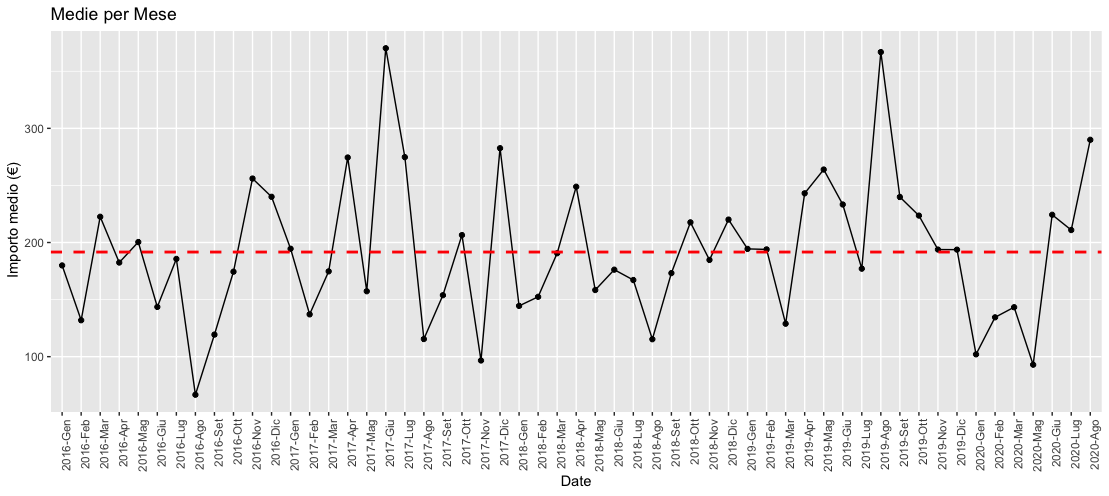
\includegraphics[scale=.3]{img/medie.png}
    \caption{Grafico di elaborazione delle medie mensili}
    \label{figure:medie}
\end{figure}
L'andamento di crescita o di stagnazione delle vendite può confermare e influenzare le strategie aziendali e gli sforzi di marketing in determinati mesi e su determinate campagne.
\subsubsection{Job 2 - Varianza di vendita per ogni mese}
La Figura \ref{figure:varianze} evidenzia l'ampiezza delle fluttuazioni mensili rispetto alla media. Un valore più alto indica una maggiore volatilità nelle vendite, mentre un valore più basso suggerisce una maggiore stabilità.
\begin{figure}[H]
    \centering
    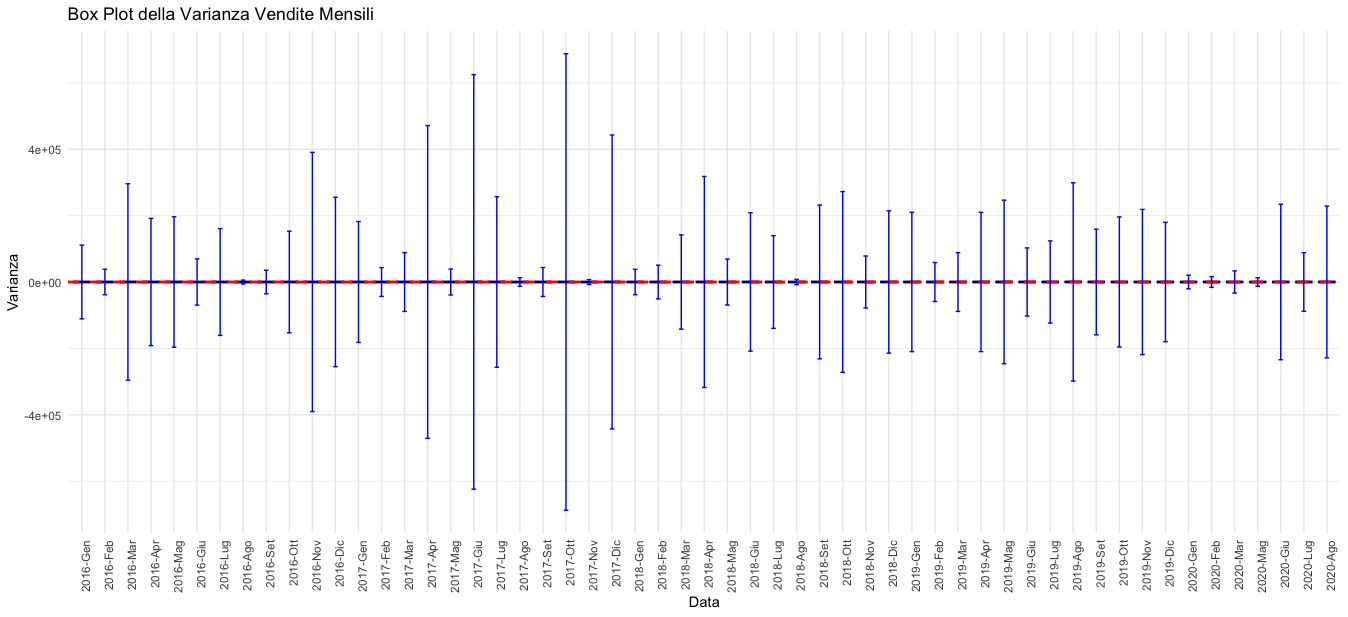
\includegraphics[scale=.25]{img/varianza.png}
    \caption{Grafico di elaborazione delle varianze mensili}
    \label{figure:varianze}
\end{figure}
Queste informazioni sono preziose per comprendere l'incertezza e l'irregolarità delle vendite durante alcuni periodi dell'anno.
\subsubsection{Job 3 e 4 - Mesi migliori e peggiori di ogni anno}
\begin{wrapfigure}{l}{0.5\textwidth}
    \centering
    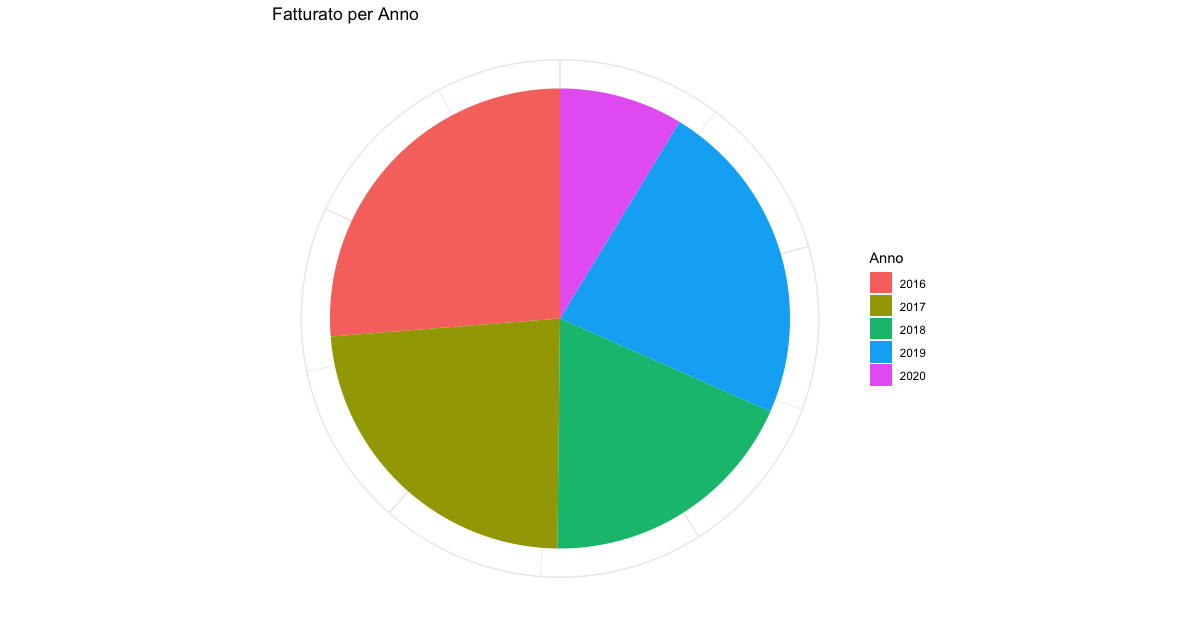
\includegraphics[width=0.5\textwidth]{img/fatturato per anno.png}
    \caption{Suddivisione fatturato per anno}
    \label{figure:fatturatoAnno}
\end{wrapfigure}

La Figura \ref{figure:fatturatoAnno} fornisce una visione globale del fatturato dell'azienda in questi anni, contestualizzando i mesi migliori e peggiori di ogni anno (sempre in riferimento alla media globale delle vendite).


L'individuazione del mese con le maggiori vendite (Figura \ref{fig:max}) è fondamentale per focalizzare l'attenzione sui fattori che hanno contribuito a questo successo, mentre l'analisi dei mesi con vendite più basse (Figura \ref{fig:min}) porta alla luce fattori di debolezza. 
\begin{figure}[H]
    \centering
    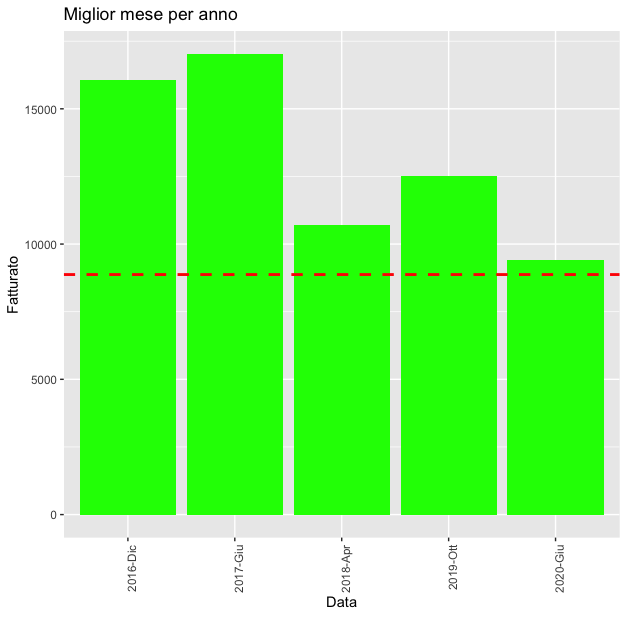
\includegraphics[scale=.3]{img/max.png}
    \caption{Migliori mesi}
        \label{fig:max}
\end{figure}
\begin{figure}[H]
    \centering
    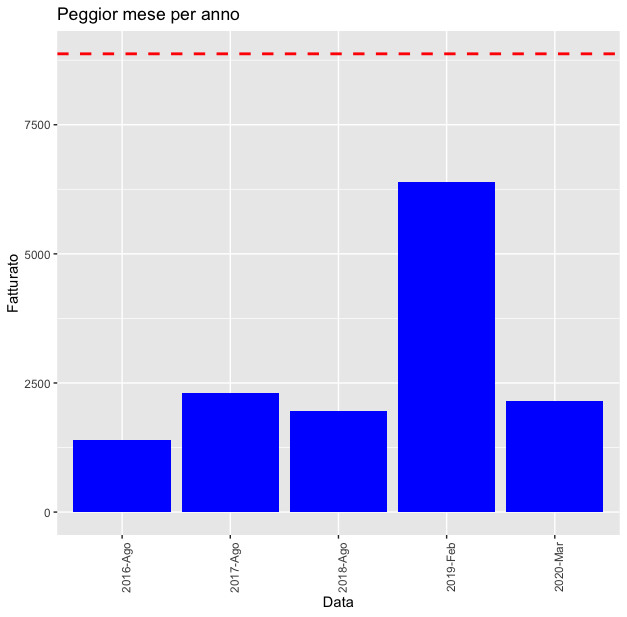
\includegraphics[scale=.3]{img/min.png}
    \caption{Peggiori mesi}
        \label{fig:min}
\end{figure}
Fattori come la stagionalità, le tendenze di mercato o le concomitanze avverse possono aver influenzato le vendite, così come potrebbero essere state implementate strategie specifiche o eventi particolari che hanno spinto le vendite al di sopra della media.
\subsubsection{Analisi}
Analizzare le condizioni e le tattiche associate ai mesi in questione può fornire lezioni preziose per guidare le future iniziative aziendali e aiutare a mitigare gli effetti negativi in situazioni simili in futuro.